%&pdflatex
\section{Debian GNU/Linux}
\textbf{Debian} è il principale argomento di questo testo. In questo paragrafo vediamo le caratteristiche distintive di questa distribuzione GNU/Linux.

Intanto, come abbiamo già detto, il fatto che sia una distribuzione \textit{GNU/Linux} ci dice che Debian ha come kernel Linux e contiene i software GNU. Di seguito sono elencate alcune delle caratteristiche che distinguono questa distribuzione:
\begin{itemize}
	\item Debian è composta unicamente da \textit{software libero}: significa che l'utente ha la libertà di eseguire, copiare, distribuire, studiare, modificare e migliorare il software;
	\item I repository di Debian contengono oltre \(43\,000\) pacchetti software;
	\item Nel tempo sono state rilasciate varie versioni di Debian: attualmente Debian è alla \textit{versione 8.6 "jessie"};
	\item Debian usa il software \texttt{apt} per gli aggiornamenti. Segue una politica di aggiornamento standard sul modello \textit{"release cycle"}. Ciò significa che tutto il software di Debian è stato preventivamente testato a lungo al fine di risolvere bug e problemi; inoltre Debian aggiorna il software per includere nuove \textit{feature} soltanto quando rilascia una nuova versione dell'intera distribuzione Debian (fix di sicurezza e bug sono sempre rilasciati il prima possibile). Vuol dire che, ad esempio, il software non viene aggiornato in Debian 8 finché non verrà rilasciata Debian 9. Questa politica serve a garantire maggior stabilità. La politica complementare si chiama \textit{"rolling release"} dove il software viene sempre aggiornato il prima possibile all'ultima versione (\textit{ArchLinux} e \textit{Gentoo} sono esempi di distribuzioni rolling);
	\item Debian usa \texttt{systemd} come \textit{init system}. L'init system è il primo programma che viene avviato su una qualsiasi distribuzione Linux: si occupa di inizializzare tutti i \textit{demoni} (programmi in background) e resta in esecuzione fino allo spegnimento del sistema. Conoscere il proprio init system è fondamentale per chiunque voglia imparare davvero a lavorare bene con un sistema Linux. \texttt{systemd} in realtà è anche molto più che un semplice init system e gestisce vari aspetti del sistema operativo --- viene criticato da una parte della comunità di Linux e del software libero (tra cui anche Linus Torvalds, Patrick Volkerding, Eric Raymond e l'autore di questo documento \texttt{:P}) per alcune scelte di design: log binari; violazione della filosofia Unix; \textit{feature creeping}; ecc\ldots. \texttt{systemd} è l'init system più diffuso;
	\item Da Debian derivano quasi tutte le altre distribuzioni Linux: Debian è, in un certo senso, la distribuzione padre di tutte le altre.
\end{itemize}
Per maggiori informazioni su Debian si veda \texttt{www.debian.org} e \texttt{en.wikipedia.org/wiki/Debian}.
%&pdflatex
\subsection{Ottenere Debian 8 "jessie"}
Ogni versione Debian ha un \textit{nome in codice}: quello di Debian 8 è \textit{"jessie"}. Attualmente Debian 8 è l'ultima versione disponibile. Quando sarà rilasciata, Debian 9 si chiamerà \textit{"stretch"} --- al momento in \textit{testing}. In quanto segue tratteremo solo \textbf{Debian 8 "jessie"}: nel caso che Debian 9 (o una versione ancora più recente) sia stata rilasciata come \textit{stable}, il lettore è invitato a scaricare la nuova versione, tenendo però presente che quanto scritto in questo testo potrebbe non essere più interamente valido.

Debian 8 "jessie" è scaricabile dal sito:

\begin{graybox}
	\texttt{https://www.debian.org/distrib/}
\end{graybox}

Nella pagina dovrebbe trovarsi quanto mostrato in Figura \vref{fig:get-debian}.

\begin{figure}[ht]
	\centering
	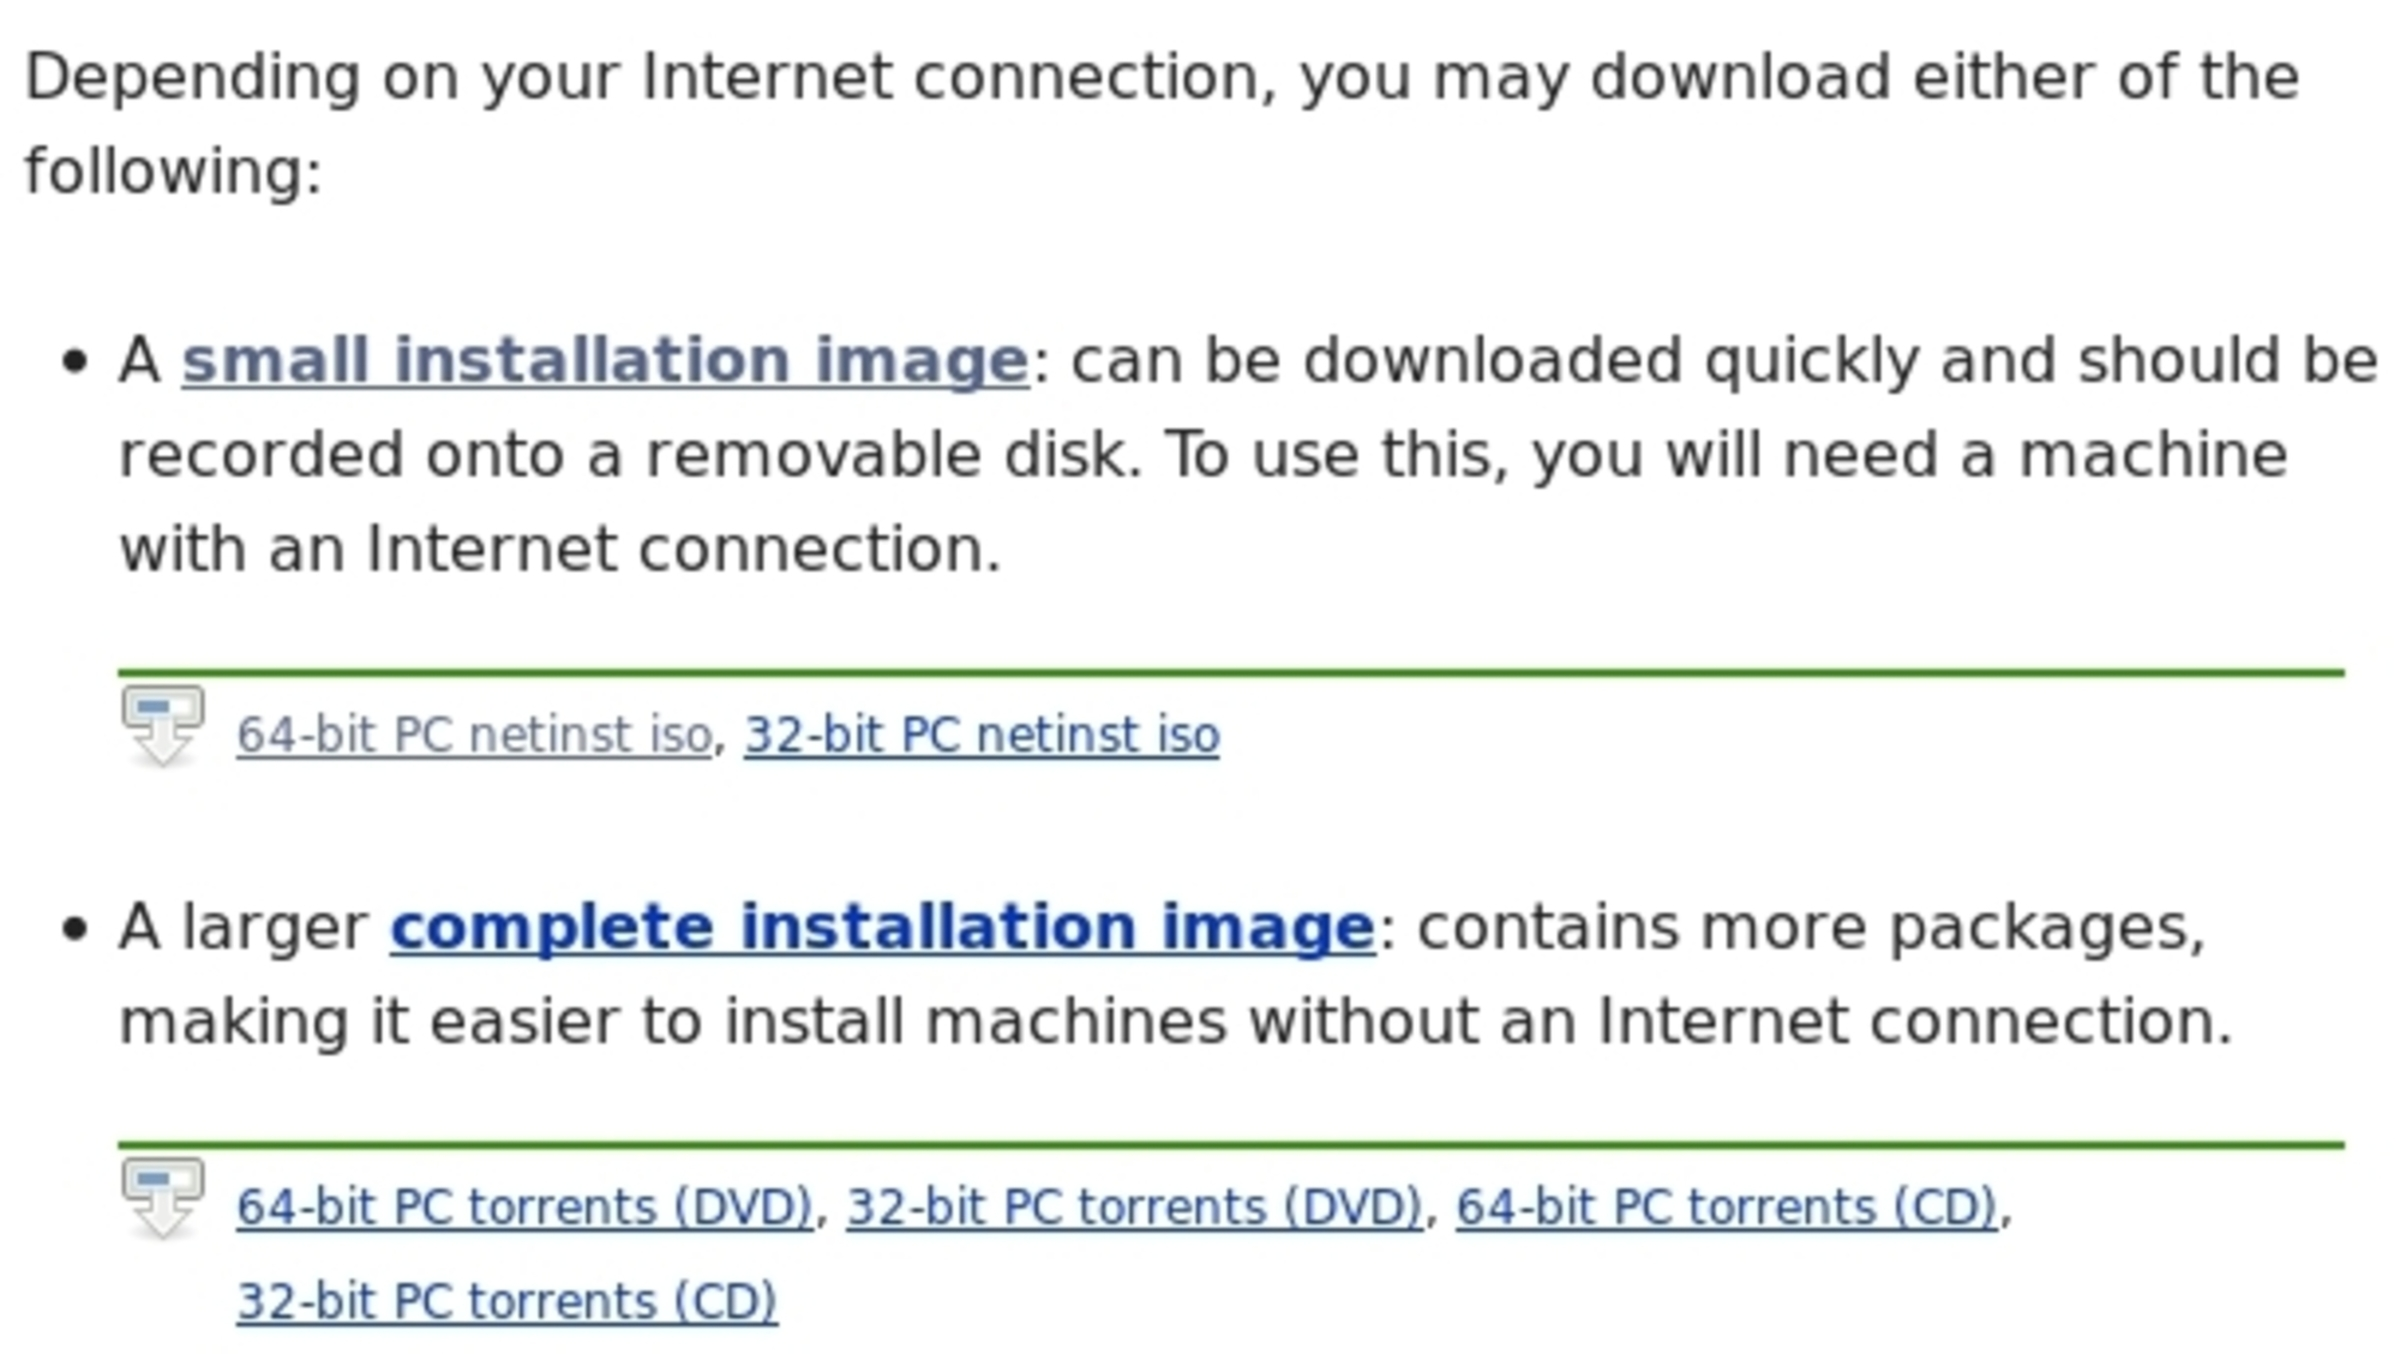
\includegraphics[resolution=600]{get-debian}
	\caption{Pagina di download di Debian}
	\label{fig:get-debian}
\end{figure}

Possiamo scegliere tra due tipi di file immagine: \textit{small (netinst)} e \textit{complete}. Non c'è alcuna differenza tra i due, se non per il fatto che il primo richiede una connessione a internet per l'installazione mentre il secondo no. Il consiglio è di utilizzare la netinst (small) in quanto richiede meno tempo per il download. Dobbiamo però anche scegliere tra due diverse versioni: \textit{64-bit PC amd64} (valida anche per architetture Intel, non inganni il nome) e \textit{32-bit PC i386}. I moderni computer hanno tutti architettura a 64 bit: l'architettura a 32 bit è obsoleta, ma in circolazione sono ancora presenti computer con questa architettura. Per determinare l'architettura del computer da Windows Vista/7 basta seguire alcuni semplici passi: \texttt{Menu Start} > \texttt{Sistema} > click destro su \texttt{Computer} > \texttt{Proprietà} e l'architettura comparirà in mezzo ad altre informazioni. Se il computer è stato acquistato con Windows 8 o successivi, allora sicuramente ha un'architettura a 64 bit; se invece è stato acquistato con Windows XP, allora sicuramente ha un'architettura a 32 bit.

\begin{graybox}
	\textbf{ATTENZIONE:} quanto detto sopra vale solo per computer con architetture Intel o AMD (le più diffuse). Debian però supporta anche altre architetture (ARM, PowerPC, MIPS, e altre ancora). Le immagini per queste architetture speciali, sono disponibili all'indirizzo:

	\texttt{https://www.debian.org/distrib/netinst}
\end{graybox}

Per poter seguire la procedura di installazione descritta nel Capitolo \vref{ch:install}, è necessario scaricare l'\textit{immagine ISO} sul proprio PC.

%&pdflatex
\subsection{Requisiti minimi di sistema}
Per poter installare e poi utilizzare Debian, sono necessari:
\begin{itemize}
	\item Almeno 256 MB di RAM (preferibilmente più di 1 GB);
	\item Almeno 10 GB di spazio su disco rigido (preferibilmente più di 30 GB).
\end{itemize}
In mancanza di questi requisiti, Debian non può essere installato.

